\documentclass{article}
\usepackage[spanish]{babel}
\usepackage[utf8]{inputenc}
\usepackage{geometry}
\usepackage{amsmath}
\usepackage{booktabs}
\usepackage{graphicx}
\usepackage{listings}
\usepackage{xcolor}
\usepackage{hyperref}

\geometry{a4paper, margin=2.5cm}
\lstset{
    basicstyle=\ttfamily\small,
    keywordstyle=\color{blue},
    numbers=left,
    numberstyle=\tiny\color{gray},
    frame=single,
    tabsize=4,
    captionpos=b,
    breaklines=true
}

\title{Simulación de Gestión de Inventarios}
\author{Diego Manuel Viera Martínez C-311}
\date{\today}

\begin{document}
\maketitle
\section{Descripción del Problema}
Consideremos una tienda que almacena cierto producto, el cual vende a un precio unitario r.
Para cubrir la demanda, el propietario de la tienda debe tener a disposición una cantidad del producto
y, siempre que el inventario disminuya, tendrá que ordenar más unidades al distribuidor.
El propietario practica una política de solicitud $(s,S)$; a saber, siempre que el inventario sea
menor que s y no haya una solicitud previa, entonces pide determinada cantidad para que
el inventario crezca hasta S, donde $s < S$. El costo de solicitud de 'y' unidades del producto para reponer el inventario 
es una función dada $c(y)$, y se necesitan L unidades de tiempo para la entrega de un pedido; el pago se realiza al momento de la entrega.
Además, la tienda paga un costo de mantenimiento del inventario de 'h' por cada artículo, por unidad de tiempo. Se sabe que si un cliente
'compra' una cantidad mayor que la del inventario solo obtiene el total que hay en el inventario en ese momento.\\

Este proyecto implementa un modelo de simulación discreta para analizar políticas de gestión de inventarios en un entorno estocástico. El sistema simula:
\begin{itemize}
    \item Llegada de clientes mediante proceso de Poisson
    \item Demanda aleatoria por cliente
    \item Costos de ordenar, mantener inventario
    \item Tiempo de entrega para reposición de stock
\end{itemize}

\subsection{Variables que describen el sistema}
\begin{itemize}
    \item Variable de tiempo: $t$
    \item Tiempo de evento de la llegada de un cliente $t_0$
    \item Tiempo de evento de la llegada de un pedido $t_1$
    \item Variables de estado:
          \begin{itemize}
            \item x: cantidad de inventario a la mano.
            \item y: cantidad solicitada.
          \end{itemize}
    \item Variables de conteo:
          \begin{itemize}
            \item C: la cantidad total de costos de los pedidos hasta t.
            \item H: la cantidad total de costos de mantenimiento de inventario hasta t.
            \item R: la cantidad total de ingresos obtenidos hasta t.
          \end{itemize}

\end{itemize}

\section{Detalles de Implementación}

\subsection*{Componentes Clave}
\subsubsection*{Variables de Estado}
\begin{itemize}
    \item $\mathbf{x}$: Inventario actual (unidades)
    \item $\mathbf{y}$: Unidades pendientes de entrega
\end{itemize}

\subsubsection*{Contadores}
\begin{itemize}
    \item $\mathbf{C}$: Costo total de pedidos
    \item $\mathbf{H}$: Costo total de almacenamiento
    \item $\mathbf{R}$: Ingresos por ventas
\end{itemize}

\subsection*{Parámetros del Modelo}
\begin{itemize}
    \item $\lambda$: Tasa de llegada de clientes (Poisson)
    \item $s$: Nivel mínimo para reordenar
    \item $S$: Nivel máximo de inventario
    \item $L$: Tiempo de entrega de pedidos
    \item $h$: Costo de almacenamiento por unidad/tiempo
    \item \texttt{c\_function}}: Función de costo de pedido
    \item \texttt{demand\_function}: Función generadora de demanda
    \item \texttt{simulation\_time}: Duración total
    \item $r$: Precio de venta por unidad
\end{itemize}

\subsection*{Mecánica de Eventos}
\subsubsection*{Llegada de Clientes}
\begin{itemize}
    \item Tiempos generados con distribución exponencial($\lambda$)
    \item Demanda por cliente: \texttt{demand\_function()}
\end{itemize}

\subsubsection*{Reabastecimiento}
\begin{itemize}
    \item Se ordena $S - x$ unidades cuando $x < s \land y = 0$
    \item Entrega después de tiempo $L$
\end{itemize}

\subsection*{Lógica de Simulación}
\begin{itemize}
    \item Cola de eventos prioritarios (heap)
    \item Cálculo proporcional de costos entre eventos
    \item Actualización de contadores al procesar cada evento
    \item Ajuste final de costos residuales al terminar
\end{itemize}

\subsection*{Retorno}
Retorna tupla con métricas clave:
\[
(\mathbf{R},\ \mathbf{C},\ \mathbf{H})
\]

\section{Resultados y Experimentos}
Para mis pruebas usé las siguientes configuraciones
    \begin{itemize}
        \item $\lambda = 2$
        \item $s \in [30 , 50]$
        \item $S = 100$
        \item $h = 0,2$
        \item $L = 30 $
        \item $c\_function = 25 + 4 * amount$
        \item $demand\_function = U(1,10)$
        \item $simulation\_time = 10080$
        \item $product\_price = 10$
    \end{itemize}
\subsection{Hallazgos de la simulación:}
    \begin{itemize}
    \item Para altos valores de lambda, o sea la tasa de llegada de clientes,puede hacer que el sistema colapse aumentando la pérdida de ventas, llegan demasiados clientes y no hay productos.
    \item Aumentar el timepo de llegada de los pedidios  $(L)$, disminuye el costo total del almacenamiento del inventario pero aumenta las pérdidas de ventas a clientes.
    \end{itemize}

\subsection{Distribución de las ganancias}
Veamos como tienen una distribución normal las ganancias con una media de 43000 unidades de ganancia:

\begin{figure}[h]
    \centering
    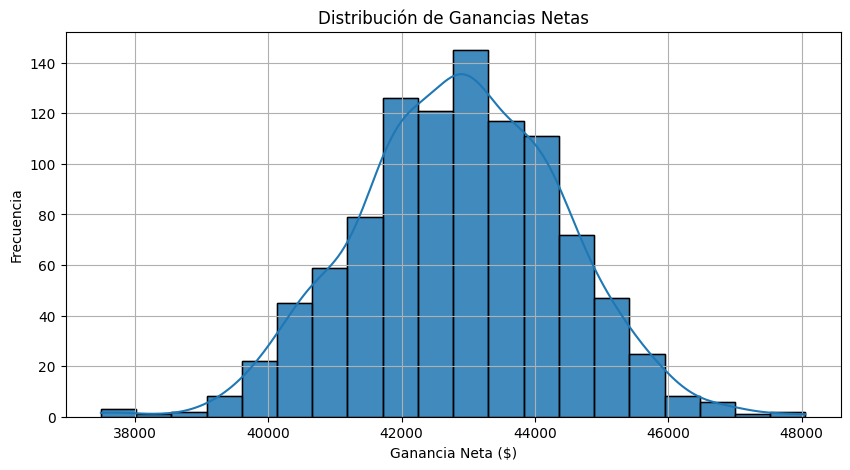
\includegraphics[width=0.8\textwidth]{images/distribution.png}
    \caption{Distribución de la ganancia promedio}
\end{figure}

\subsection{Hipótesis de los resultados}
    \begin{itemize}
        \item Aumentar la capacidad mínima del inventario aumenta significativamente el costo de los pedidios.
        \item Aumentar la capacidad mínima del inventario aumenta significativamente el costo del almacenamiento.
    \end{itemize}
\subsection{Experimentos realizados para validar las hipótesis}
Para validar mis hipótesis utilicé una prueba t student para muestras independientes, para comparar las distribuciones de costos entre ambos escenarios. Esta prueba evalúa si las diferencias observadas en las medias son estadísticamente significativas. Se realizaron 100 simulaciones con un mínimo de capacidad de 30 unidades y otras 100 simulaciones con un mínimo de capacidad de 50 unidades y en efecto existe una gran diferencia entre ambas configuraciones, con la capacidad mínima mayor se obtienen mayores gastos tanto de pedidos como de almacén.

\begin{figure}[h]
    \centering
    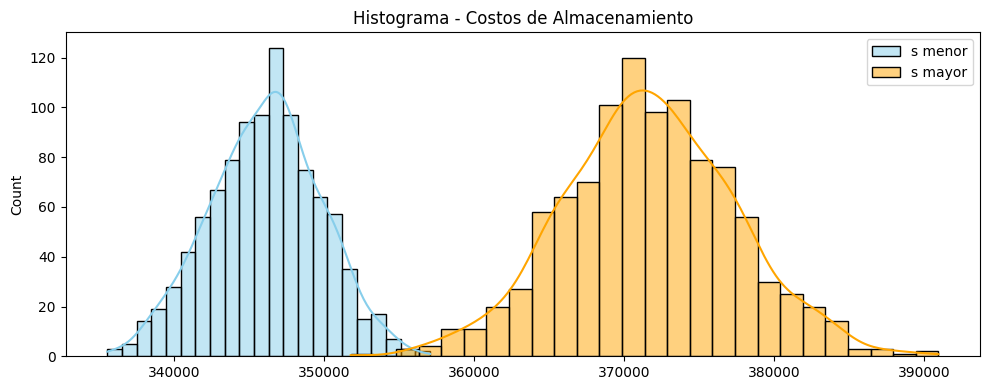
\includegraphics[width=0.8\textwidth]{images/CostosAlmacen.png}
    \caption{Comparación de costos del almacén}
\end{figure}

\begin{figure}[h]
    \centering
    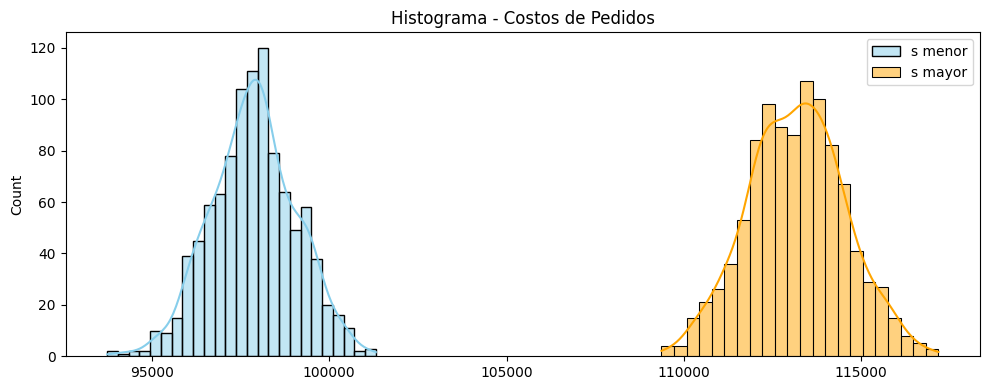
\includegraphics[width=0.8\textwidth]{images/CostosPedidos.png}
    \caption{Comparación de costos de pedidos}
\end{figure}

\section{Modelo Matemático}
\begin{itemize}
    \item $Ingresos = \sum_{i=1}^{N} \min(d_i, I(t_i)) * r$
    \item $Costos\_de\_Almacén = h \cdot \int_{0}^{T} I(t) dt$
    \item $Costos\_de\_Pedido = \sum_{j=1}^{M} C(q_j)$
    \item $Ganancia\_neta= Ingresos - Costos\_de\_Pedidos - Costos\_de\_Almacén$
\end{itemize}

donde:
\begin{itemize}
    \item $I(t)$: Cantidad de unidades en el inventario en el tiempo $t$
    \item $d_i$: Demanda del i-ésimo cliente
    \item $q_j$: Cantidad de unidades que se ordenó en el j-ésimo pedido.
    \item $r$: Precio del producto
\end{itemize}

\section{Conclusiones}
El modelo de simulación desarrollado permite analizar rigurosamente el impacto de la política (s, S) en los costos operativos y el nivel de servicio. Los experimentos demostraron que ajustar el nivel mínimo de reorden (s) tiene efectos estadísticamente significativos en los costos de pedidos y almacenamiento, validados mediante pruebas t de Student. Se evidenció un claro equilibrio entre mantener altos niveles de inventario (para evitar ventas perdidas) y minimizar costos.

\end{document}